\documentclass{standalone}
\usepackage{pgfplots}
\pgfplotsset{compat = 1.15}
\begin{document}
    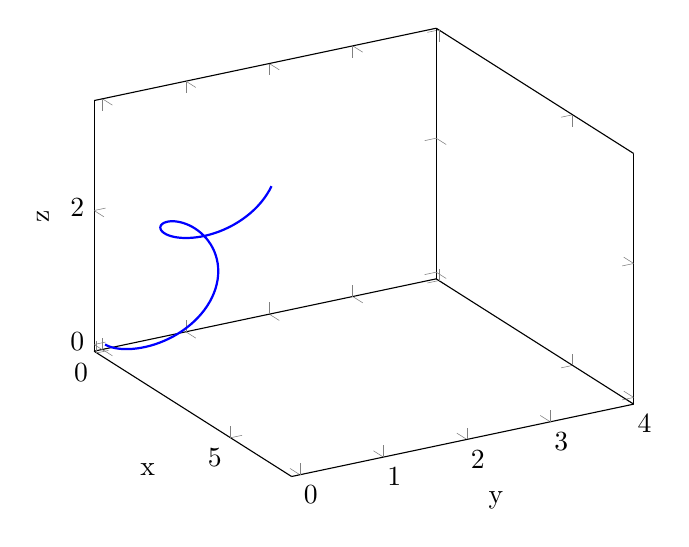
\begin{tikzpicture}
        \begin{axis} [
            view = {60}{30},
            xlabel = {x},
            ylabel = {y},
            zlabel = {z},
            ymin = -0.1,
            ymax = 4,
            xmin = -0.1,
            xmax = 2*pi + 1,
            zmin = -0.1,
            zmax = pi + 0.5]
            \addplot3 [thick, blue, domain = 0:2*pi, samples = 100, samples y = 0] ({sin(deg(sqrt(2)*x))/(2*sqrt(2)) + x/2}, -{cos(deg(sqrt(2)*x))/2 + 1/2}, -{sin(deg(sqrt(2)*x))/(2*sqrt(2)) + x/2});
        \end{axis}
    \end{tikzpicture}
    
    \begin{tikzpicture}
        \begin{axis} [
            view = {90}{63},
            xlabel = {x},
            ylabel = {y},
            zlabel = {z},
            ymin = -0.1,
            ymax = 4,
            xmin = -0.1,
            xmax = 2*pi + 1,
            zmin = -0.1,
            zmax = pi + 0.5]
            \addplot3 [thick, blue, domain = 0:2*pi, samples = 100, samples y = 0] ({sin(deg(sqrt(2)*x))/(2*sqrt(2)) + x/2}, -{cos(deg(sqrt(2)*x))/2 + 1/2}, -{sin(deg(sqrt(2)*x))/(2*sqrt(2)) + x/2});
        \end{axis}
    \end{tikzpicture}
    
\end{document}